\chapter{Projects}

\section{STM32 IMU}
\subsection{PModNav}
The purpose is to get the \texttt{roll}, \texttt{pitch} and \texttt{yaw} from the PModNav to plot a 3D visualization of the IMU. The final purpose of it is to create log files from the orientation and attitude of the drone in real-time. By combining data from accelerometers, gyroscopes and magnetometers, an IMU can provide information about the object's position, orientation and angular velocity. This is crucial for tasks such as safety deployement or drone tracking.
The STM32-L4796ZG recovers the value of the sensors from the \texttt{PModNav} via \texttt{SPI Bus} and transmits them to the HMI via \texttt{UART} connection.
\begin{figure}[H]
    \centering
    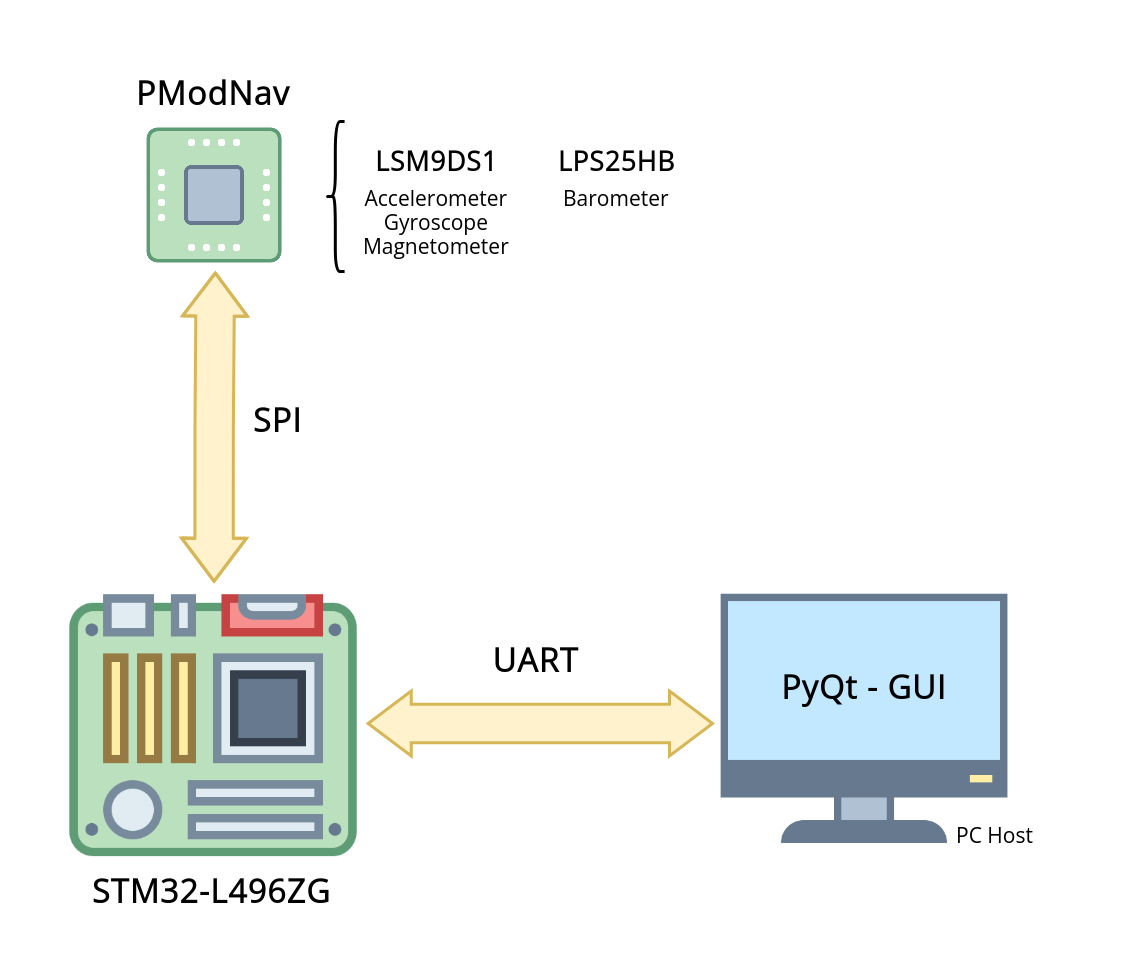
\includegraphics[width=0.65\linewidth]{./projects/pmodnav/com.png}
    \caption{Project communication overview}
\end{figure}

\subsubsection{Hardware}
The PModNav module is equipped with the \texttt{LSM9DS1}\cite{LSM9DS1_digilent_lib} sensor, offering 10-\gls{dof} functionality. It integrates a 3-axis accelerometer, 3-axis gyroscope, 3-axis magnetometer, and an LPS25HB digital barometer. This comprehensive sensor suite allows users to obtain orientation-related data and determine the precise position and heading of the module. The module supports various full-scale options for linear acceleration, angular rate, and magnetic field measurements. It follows the Digilent Interface Specification Type 2A and utilizes a 12-pin Pmod connector with an SPI interface.

\subsubsection{Software and Development Environment}
The development environment for the PModNav project is STM32 CubeIDE. The documentation references project sources, including code snippets and libraries, such as the PModNav driver and Madgwick's filter implementation. 

\subsubsection{Data Processing}
The project outlines two approaches for deriving object attitudes: Euler angles and quaternions. Euler angles are obtained through the integration of angular velocity and provide information about the roll, pitch, and yaw of an object. However, a challenge known as \texttt{Gimbal Lock}\cite{gimbal_lock} arises when using Euler angles directly, resulting in a loss of a degree of freedom when two axes of rotation overlap. To overcome this, quaternions are introduced as a mathematical representation of displacement and rotation. They effectively resolve the Gimbal Lock issue and provide a more robust solution for determining attitudes.
\begin{figure}[H]
    \centering
    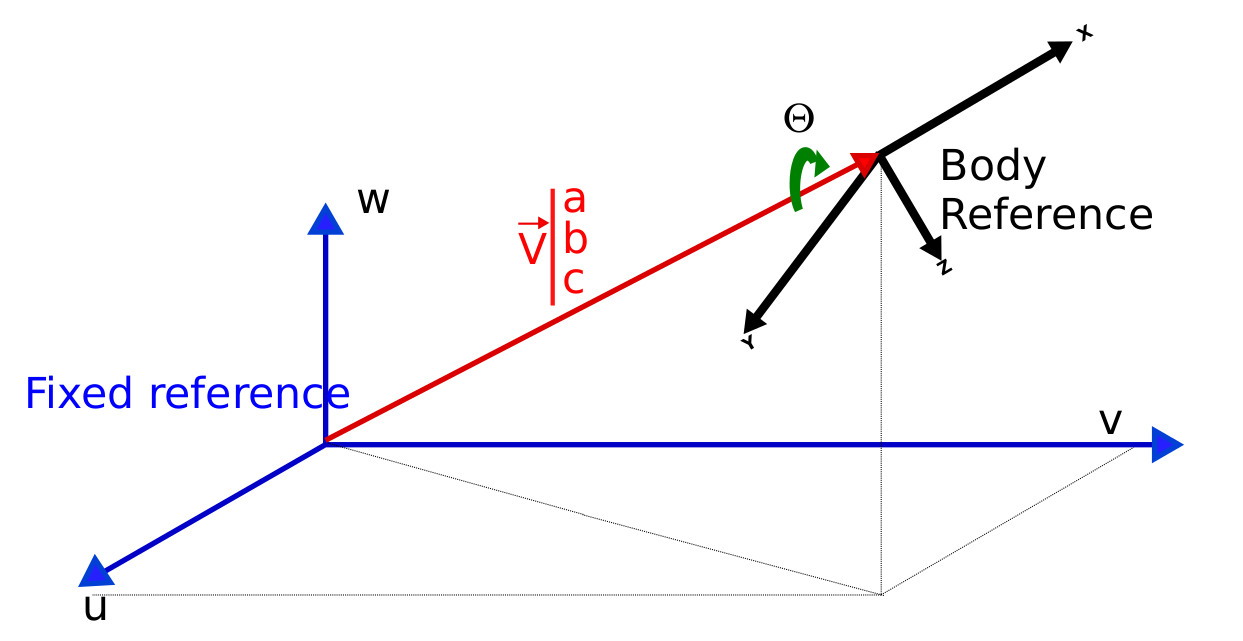
\includegraphics[width=0.65\linewidth]{./projects/pmodnav/quaternions.png}
    \caption{Quaternion representation}
\end{figure}
$$ Q = [q_0, q_1, q_2, q_3 ] $$
$$ Q = \big[cos(\frac{\theta}{2}), a.sin(\frac{\theta}{2}), b.sin(\frac{\theta}{2}), c.sin(\frac{\theta}{2})\big] $$
At each \texttt{Te}, we can calculate the new value of the quaternion vector from the velocity :
$$ Q_{k+1} = Q_k+\frac{1}{2}.T_e.\omega_k.Q_k $$
For cheap IMUs, it is unavoidable to perform a data fusion to make the accelerometer compensate for the gyroscope defect. If using a \texttt{Kalman filter}\cite{kalman_filter} is possible, there are other (faster) algorithms like Madgwick's. The idea is to compensate for the gyroscope measurement error by modulating its values by the result of a comparison between an estimate of the gravity field and the measured gravity field (with the accelerometer).
\hfill \break
\boitesimple{\underline{Note:} Only 6 \gls{dof} from the accelerometer and gyroscope have been use to this project due to too sensitive and hard to calibrate data from the magnetometer}

\begin{figure}[H]
    \centering
    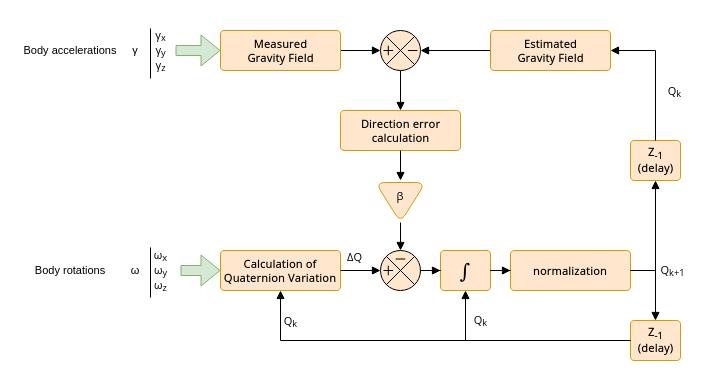
\includegraphics[width=0.9\linewidth]{./projects/pmodnav/madgwick.png}
    \caption{Madgwick filter schematic}
\end{figure}
I decided to use the most popular open source algorithm to compute rotations, the \texttt{Madgwick's algorithm}\cite{Madgwick}. This calculation updates the quaternion, from which the attitudes (Euler angles) can be calculated.
\begin{figure}[H]
    \centering
    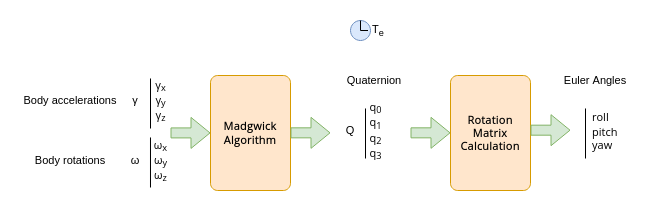
\includegraphics[width=0.9\linewidth]{./projects/pmodnav/madgwick_applied.png}
    \caption{Data transform schematic}
\end{figure}

Calculation of the Euler Angles from the rotation matrix :

\begin{minipage}[H]{0.5\textwidth}
    \vspace{0pt}
    \begin{align*}
        R_{12} &= 2(q_1q_2+q_0q_3) \\
        R_{22} &= q_0^2+q_1^2-q_2^2-q_3^2 \\
        R_{31} &= 2(q_0q_1+q_2q_3) \\
        R_{32} &= 2(q_1q_3-q_0q_2) \\
        R_{33} &= q_0^2-q_1^2-q_2^2+q_3^2 \\
    \end{align*}
\end{minipage}%
\begin{minipage}[H]{0.5\textwidth}
    \vspace{0pt}
    \begin{align*}
        \text{roll}  &= \mathrm{atan2}(R_{31},R_{33}) \\
        \text{pitch} &= \sin(R_{32}) \\
        \text{yaw}   &= \mathrm{atan2}(R_{12},R_{22}) \\
    \end{align*}
\end{minipage}

\subsection{Graphical User Interface}
Additionally, a graphical user interface \gls{gui} is provided, leveraging \texttt{PyQt5}\cite{pyqt5} and \texttt{PyOpenGL}\cite{pyopengl} modules. The \gls{gui} manages the main window and handles OpenGL object management. It offers features like port selection and serial communication. The received data is displayed in a textbox within the \gls{gui}, facilitating real-time monitoring and analysis.
Here is how the \gls{gui} is threaded :
\begin{figure}[H]
    \centering
    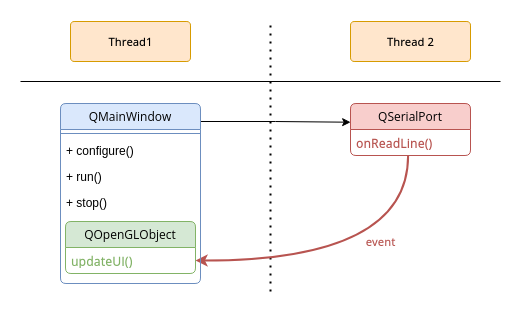
\includegraphics[width=0.65\linewidth]{./projects/pmodnav/gui_threads.png}
    \caption{Python \gls{gui} threads schematic}
\end{figure}
The use is rather simple for the communication configuration (\colorbox{cyan}{cyan box}) :
\begin{itemize}
    \item the port
    \item the baud rate
    \item the number of bits per frame
    \item the number of stop bits
    \item the parity
    \item the flow control
\end{itemize}
\begin{figure}[H]
    \centering
    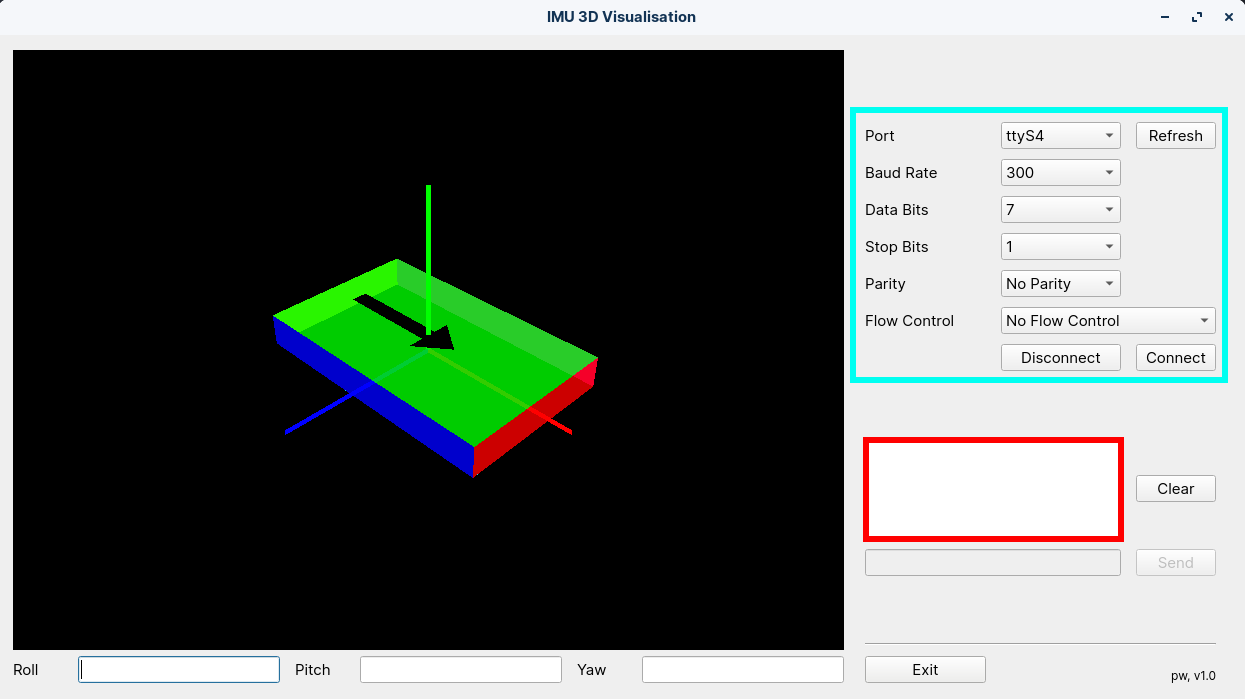
\includegraphics[width=0.65\linewidth]{./projects/pmodnav/gui_window.png}
    \caption{Python \gls{gui} window screenshot}
\end{figure}
Then click on \texttt{Connect} to start the serial communication. Every received line appeared in the textBox (\colorbox{red}{red box}).

\subsubsection{Final result}
\begin{figure}[H]
    \centering
        \href{https://youtu.be/qVYGa0Z1S-M}{
            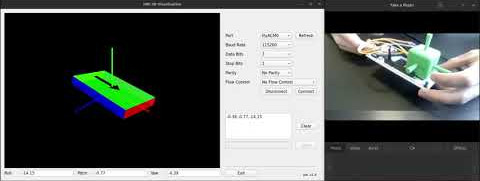
\includegraphics[width=\linewidth]{./projects/pmodnav/pmodnav_thumbnail.jpg}
        }
        \caption{3D IMU Visualizer demo}
\end{figure}

\subsection{Real-Time Operating System}
Drones, or unmanned aerial vehicles, have gained significant popularity and application across various industries. As drones become more advanced and complex, it is crucial to incorporate reliable systems for data logging and analysis. One such system is a blackbox, which serves as a flight data recorder for drones. Here are the reason of having a blackbox on a drone :
\begin{itemize}
    \item \underline{Flight Data Logging:} A blackbox records various flight parameters and sensor data during drone flights. This data can include information such as GPS coordinates, altitude, speed, battery voltage, motor RPM, control inputs, and more. Analyzing this data can provide valuable insights into the drone's performance, diagnose issues, and improve flight characteristics.
    \item \underline{Accident Investigation:} In the event of a drone crash or incident, a blackbox can provide crucial data for accident investigation and analysis. It helps in understanding the sequence of events leading up to the accident, identifying any anomalies or failures, and determining the cause of the incident. This information can be used for troubleshooting, improving safety measures, and preventing similar incidents in the future.
    \item \underline{System Optimization:} By analyzing the flight data recorded by the blackbox, drone manufacturers and developers can optimize the drone's performance, stability, and efficiency. They can fine-tune flight control algorithms, evaluate sensor accuracy, and identify areas for improvement in terms of power consumption, aerodynamics, and overall system design.
    \item \underline{Regulatory Compliance:} In some countries, drone operations may be subject to regulatory requirements. Flight data recording and analysis can help demonstrate compliance with regulations, such as maintaining safe distances from restricted areas or operating within altitude limits. The recorded data can serve as evidence of adherence to guidelines and regulations set by aviation authorities.
\end{itemize}
\hfill \break
Overall, using a blackbox on a drone provides valuable data for performance analysis, troubleshooting, safety improvement, and compliance with regulations. It allows drone operators, manufacturers, and researchers to gain insights into flight characteristics and make informed decisions for enhancing drone performance and safety.
\\ \\
The best way to implement it is to use \gls{rtos}, they provide a highly accurate sampling period and easy task management for every kind of application. In my case, I have 2 tasks that should run independantly :
\begin{table}[H]
    \centering
    \begin{tabular}{|c||c|c|c|}
    \hline
    Task Name & Frequency {[}Hz{]} & Duration {[}ms{]} & Priority \\ \hline
    IMU\_Step & 100 Hz             & $\sim$1 ms        & High     \\ \hline
    Data\_Log   & 4 Hz             & $\sim$175 ms      & Low      \\ \hline
    \end{tabular}
    \caption{\gls{rtos} tasks description}
    \label{table:tasks_details}
\end{table}

Beacause \texttt{IMU\_Step}'s priority is higher than \texttt{Data\_Log}'s priority and I want it to run at 100 Hz, I decided to use a semaphore on timer interuption to release the \texttt{IMU\_Step} task.
\begin{figure}[H]
    \centering
    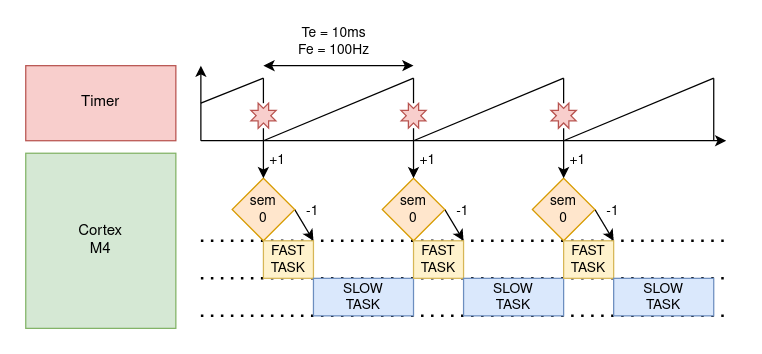
\includegraphics[width=0.75\linewidth]{./projects/pmodnav/rtos_overall.png}
    \caption{RTOS overall chart}
    \label{fig:rtos_overall}
\end{figure}

Here is the temporal plot of both tasks :
\begin{figure}[H]
    \centering
    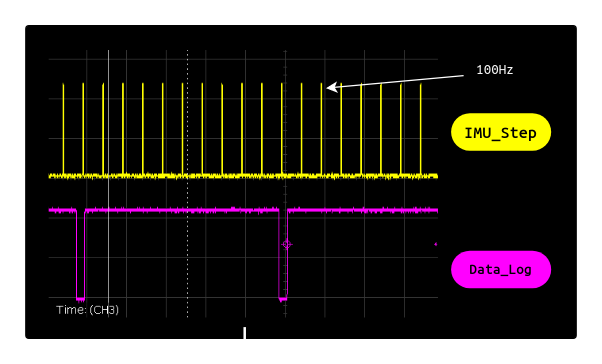
\includegraphics[width=0.75\linewidth]{./projects/pmodnav/osci_screen.png}
    \caption{Oscilloscope tasks measurements}
    \label{fig:osci_tasks}
\end{figure}

\boitesimple{\underline{Note:}Everything work has planned up to 200 Hz for the IMU and the UART data log. However, it will be a big improvement to add a SDCard data storage to get all data}

\subsubsection{SD Card handler}
The next improvment is to add the SDCard store feature, here is a Figure~\ref{fig:project_store} to how the byte communication should be done for the next step.
It's pretty simple : all typed data are converted to bytes to reduce the memory size of it. The \texttt{UART} connection works and allow to send all data at $\sim$50 Hz and the SDCard store system should use the \texttt{SPI} or \texttt{SDMMC} connection.
\begin{figure}[H]
    \centering
    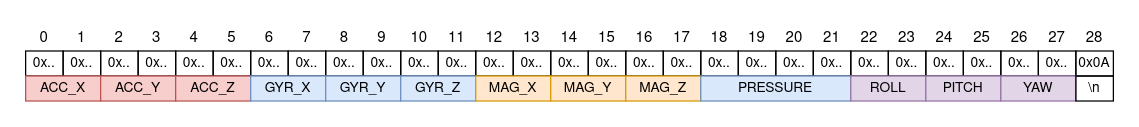
\includegraphics[width=\linewidth]{./projects/pmodnav/frame_description.png}
    \caption{Data frame as byte format}
    \label{fig:frame_description}
\end{figure}

\begin{figure}[H]
    \centering
    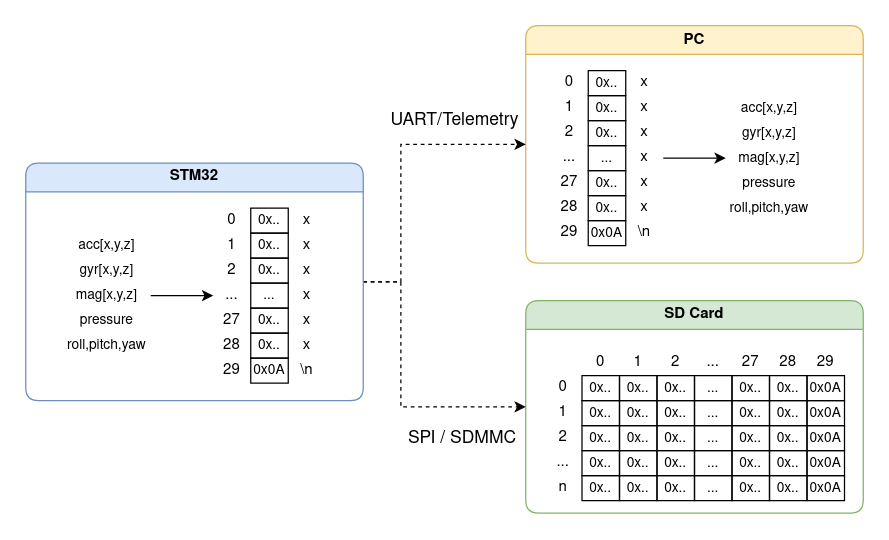
\includegraphics[width=0.75\linewidth]{./projects/pmodnav/project_store.png}
    \caption{STM32 data communication and storage}
    \label{fig:project_store}
\end{figure}

\section{LogViewer}
The objective of a log viewer application is to facilitate the efficient viewing and analysis of log data generated by systems or applications.
This scientific report highlights the key goals and functionality of a log viewer, which includes log visualization, search and filtering capabilities, log analysis and insights, integration with other tools, and customization options.
\subsection{Sensors tests}
Before using any sensors, make sure they work properly, that communication is correct and that measurements are consistent with the reality of the environment.
To check all these prerequisites, it's often easiest to use the manufacturer's proprietary software, which is robust, reliable and easy to use.

A few parameters need to be modified to enable the 8 distance sensors and their data to be taken into account by the collision avoidance built-in algorithm.
\\ \\
Here is the final configuration for a minimum effective distance of 3 meters between the drone and obstacles and a maximum effective distance of 5 meters :

\begin{table}[H]
    \centering
    \begin{subfigure}[b]{0.475\textwidth}
        \raggedright
        \resizebox{1.4\linewidth}{!}{%
            \begin{tabular}[b]{|l||l|l|}
            \hline
                              & TowerEvo & Description                 \\
            \hline
            PRX\_ORIENT       & 0        & Default                     \\
            PRX\_TYPE         & 6        & TeraRangerTowerEvo          \\
            SERIAL\_BAUD      & 921600   & Serial baud                 \\
            SERIAL\_PROTOCOLE & 11       & Lidar 360 deg               \\
            AVOID\_ANGLE      & 1300     & Max  lean angle             \\
            AVOID\_BEHAVE     & 1        & Stop when obstacle detected \\
            AVOID\_DIST\_MAX  & 5        & Max distance avoidance      \\
            AVOID\_ENABLE     & 3        & Enable drone reaction       \\
            AVOID\_MARGIN     & 3        & Min distance avoidance      \\
            \hline
            \end{tabular}%
        }
        \caption{Ardupilot flight controller configuration}
        \label{table:fc_config}
    \end{subfigure}
    \hfill
    \begin{subfigure}[b]{0.475\textwidth}
        \raggedleft
        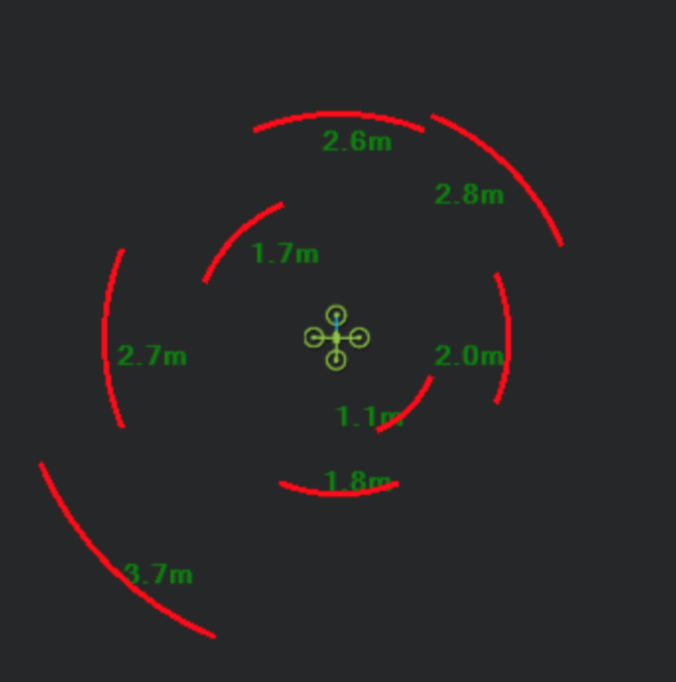
\includegraphics[height=0.56\linewidth]{./projects/logviewer/mission_planner_tower_evo.png}
        \caption{Data acquisition acknowledgement}
    \end{subfigure}
    \caption{Ardupilot configuration \& data acknowledgement} 
\end{table}


\subsection{Sensors Integration and drone flight}
\begin{figure}[H]
    \centering
    \begin{subfigure}[b]{0.475\textwidth}
        \centering
        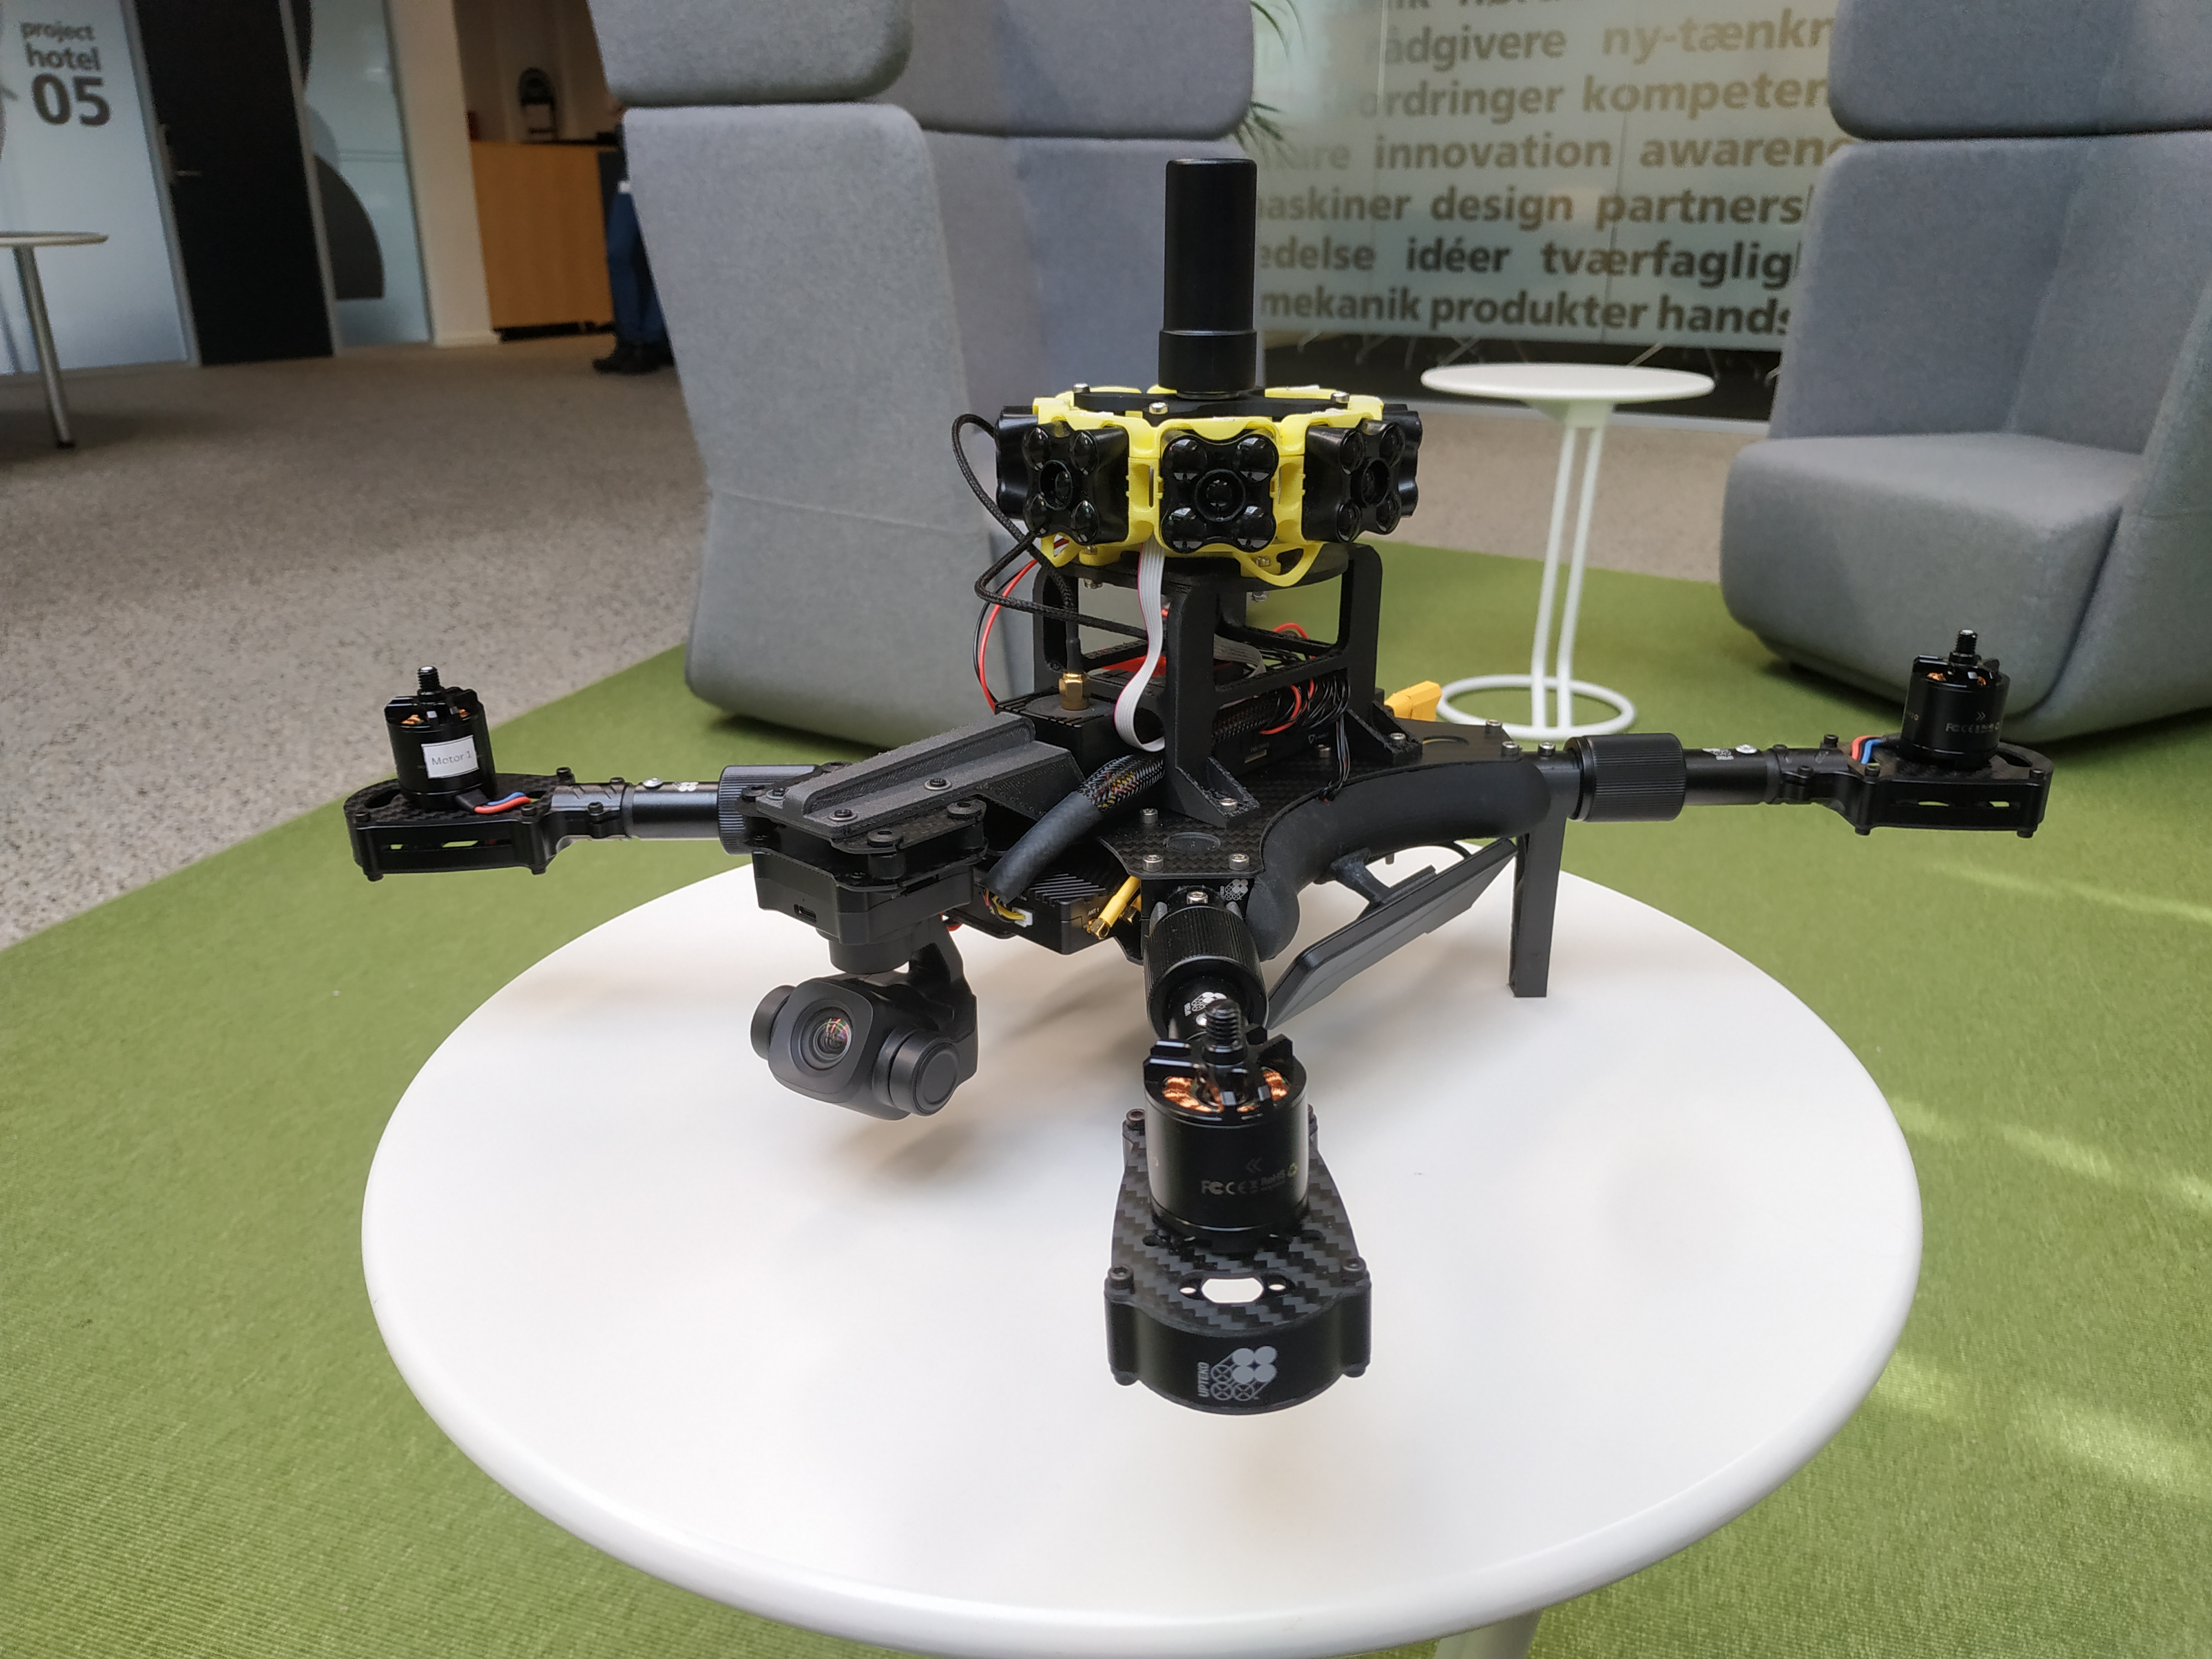
\includegraphics[width=\textwidth]{./projects/logviewer/drone_fl_view.jpg}
        \caption{Front left view}
    \end{subfigure}
    \hfill
    \begin{subfigure}[b]{0.475\textwidth}  
        \centering 
        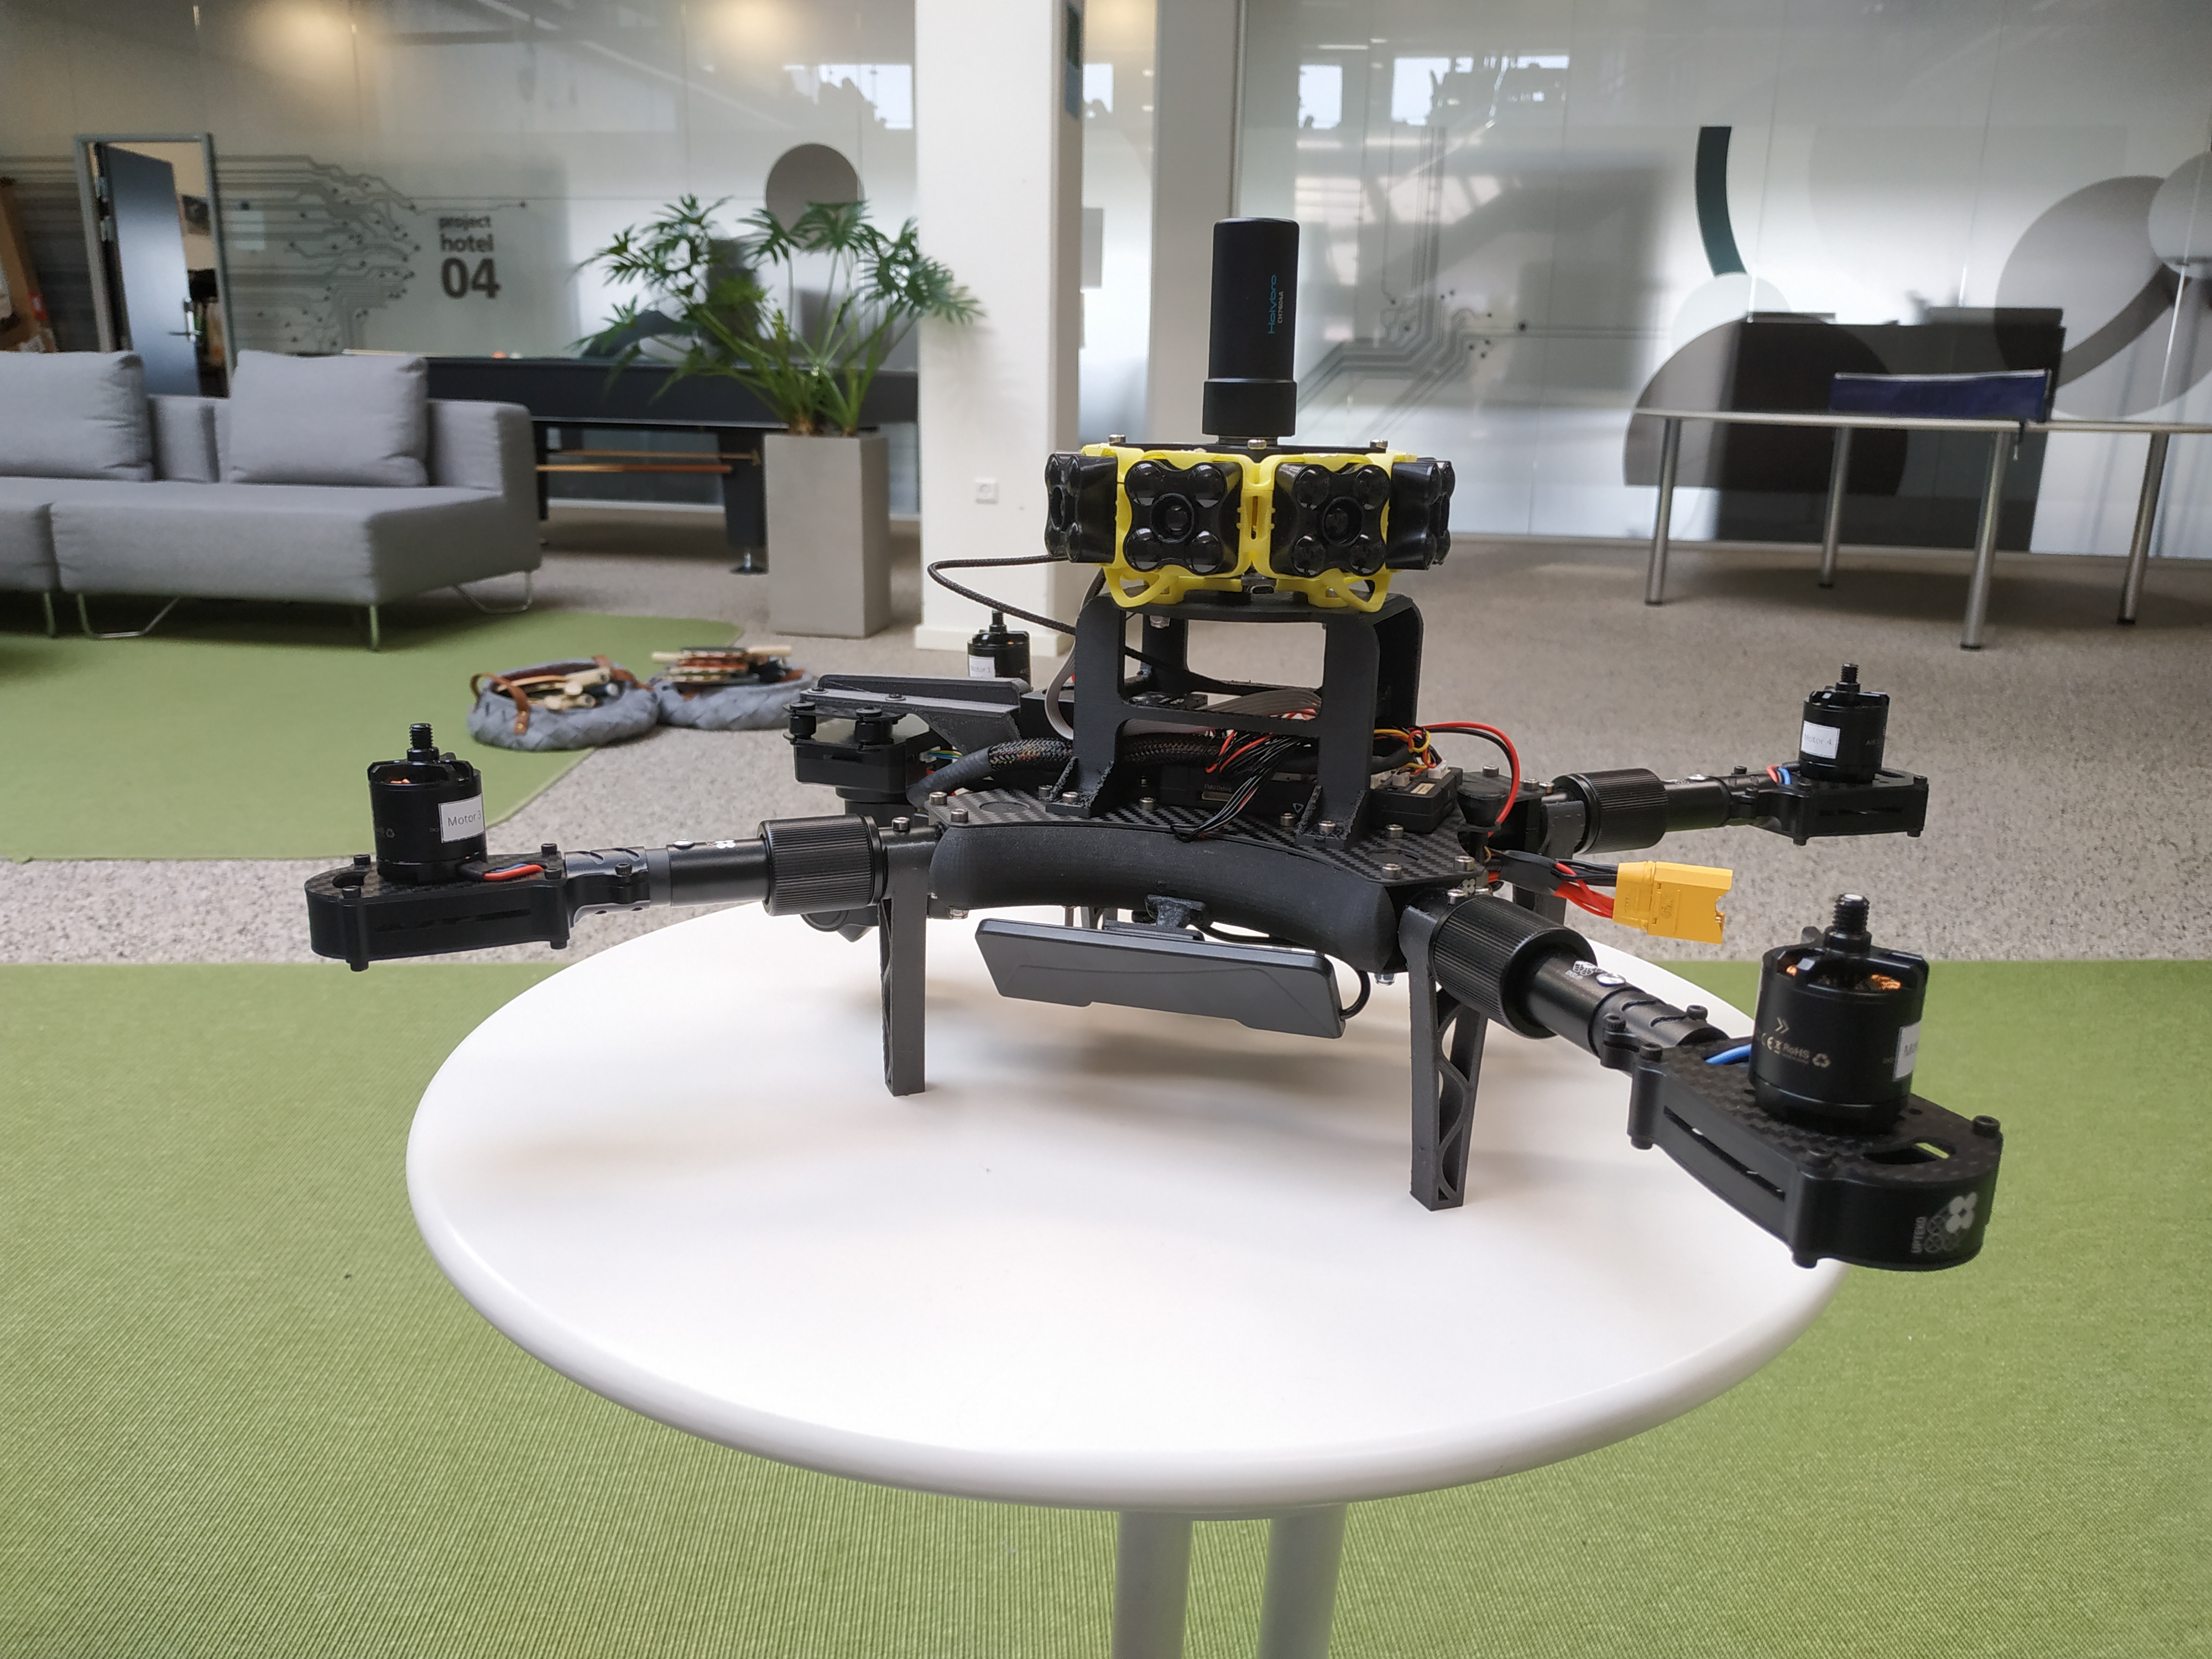
\includegraphics[width=\textwidth]{./projects/logviewer/drone_l_view.jpg}
        \caption{Left view}
    \end{subfigure}
    \vskip\baselineskip
    \begin{subfigure}[b]{0.475\textwidth}   
        \centering 
        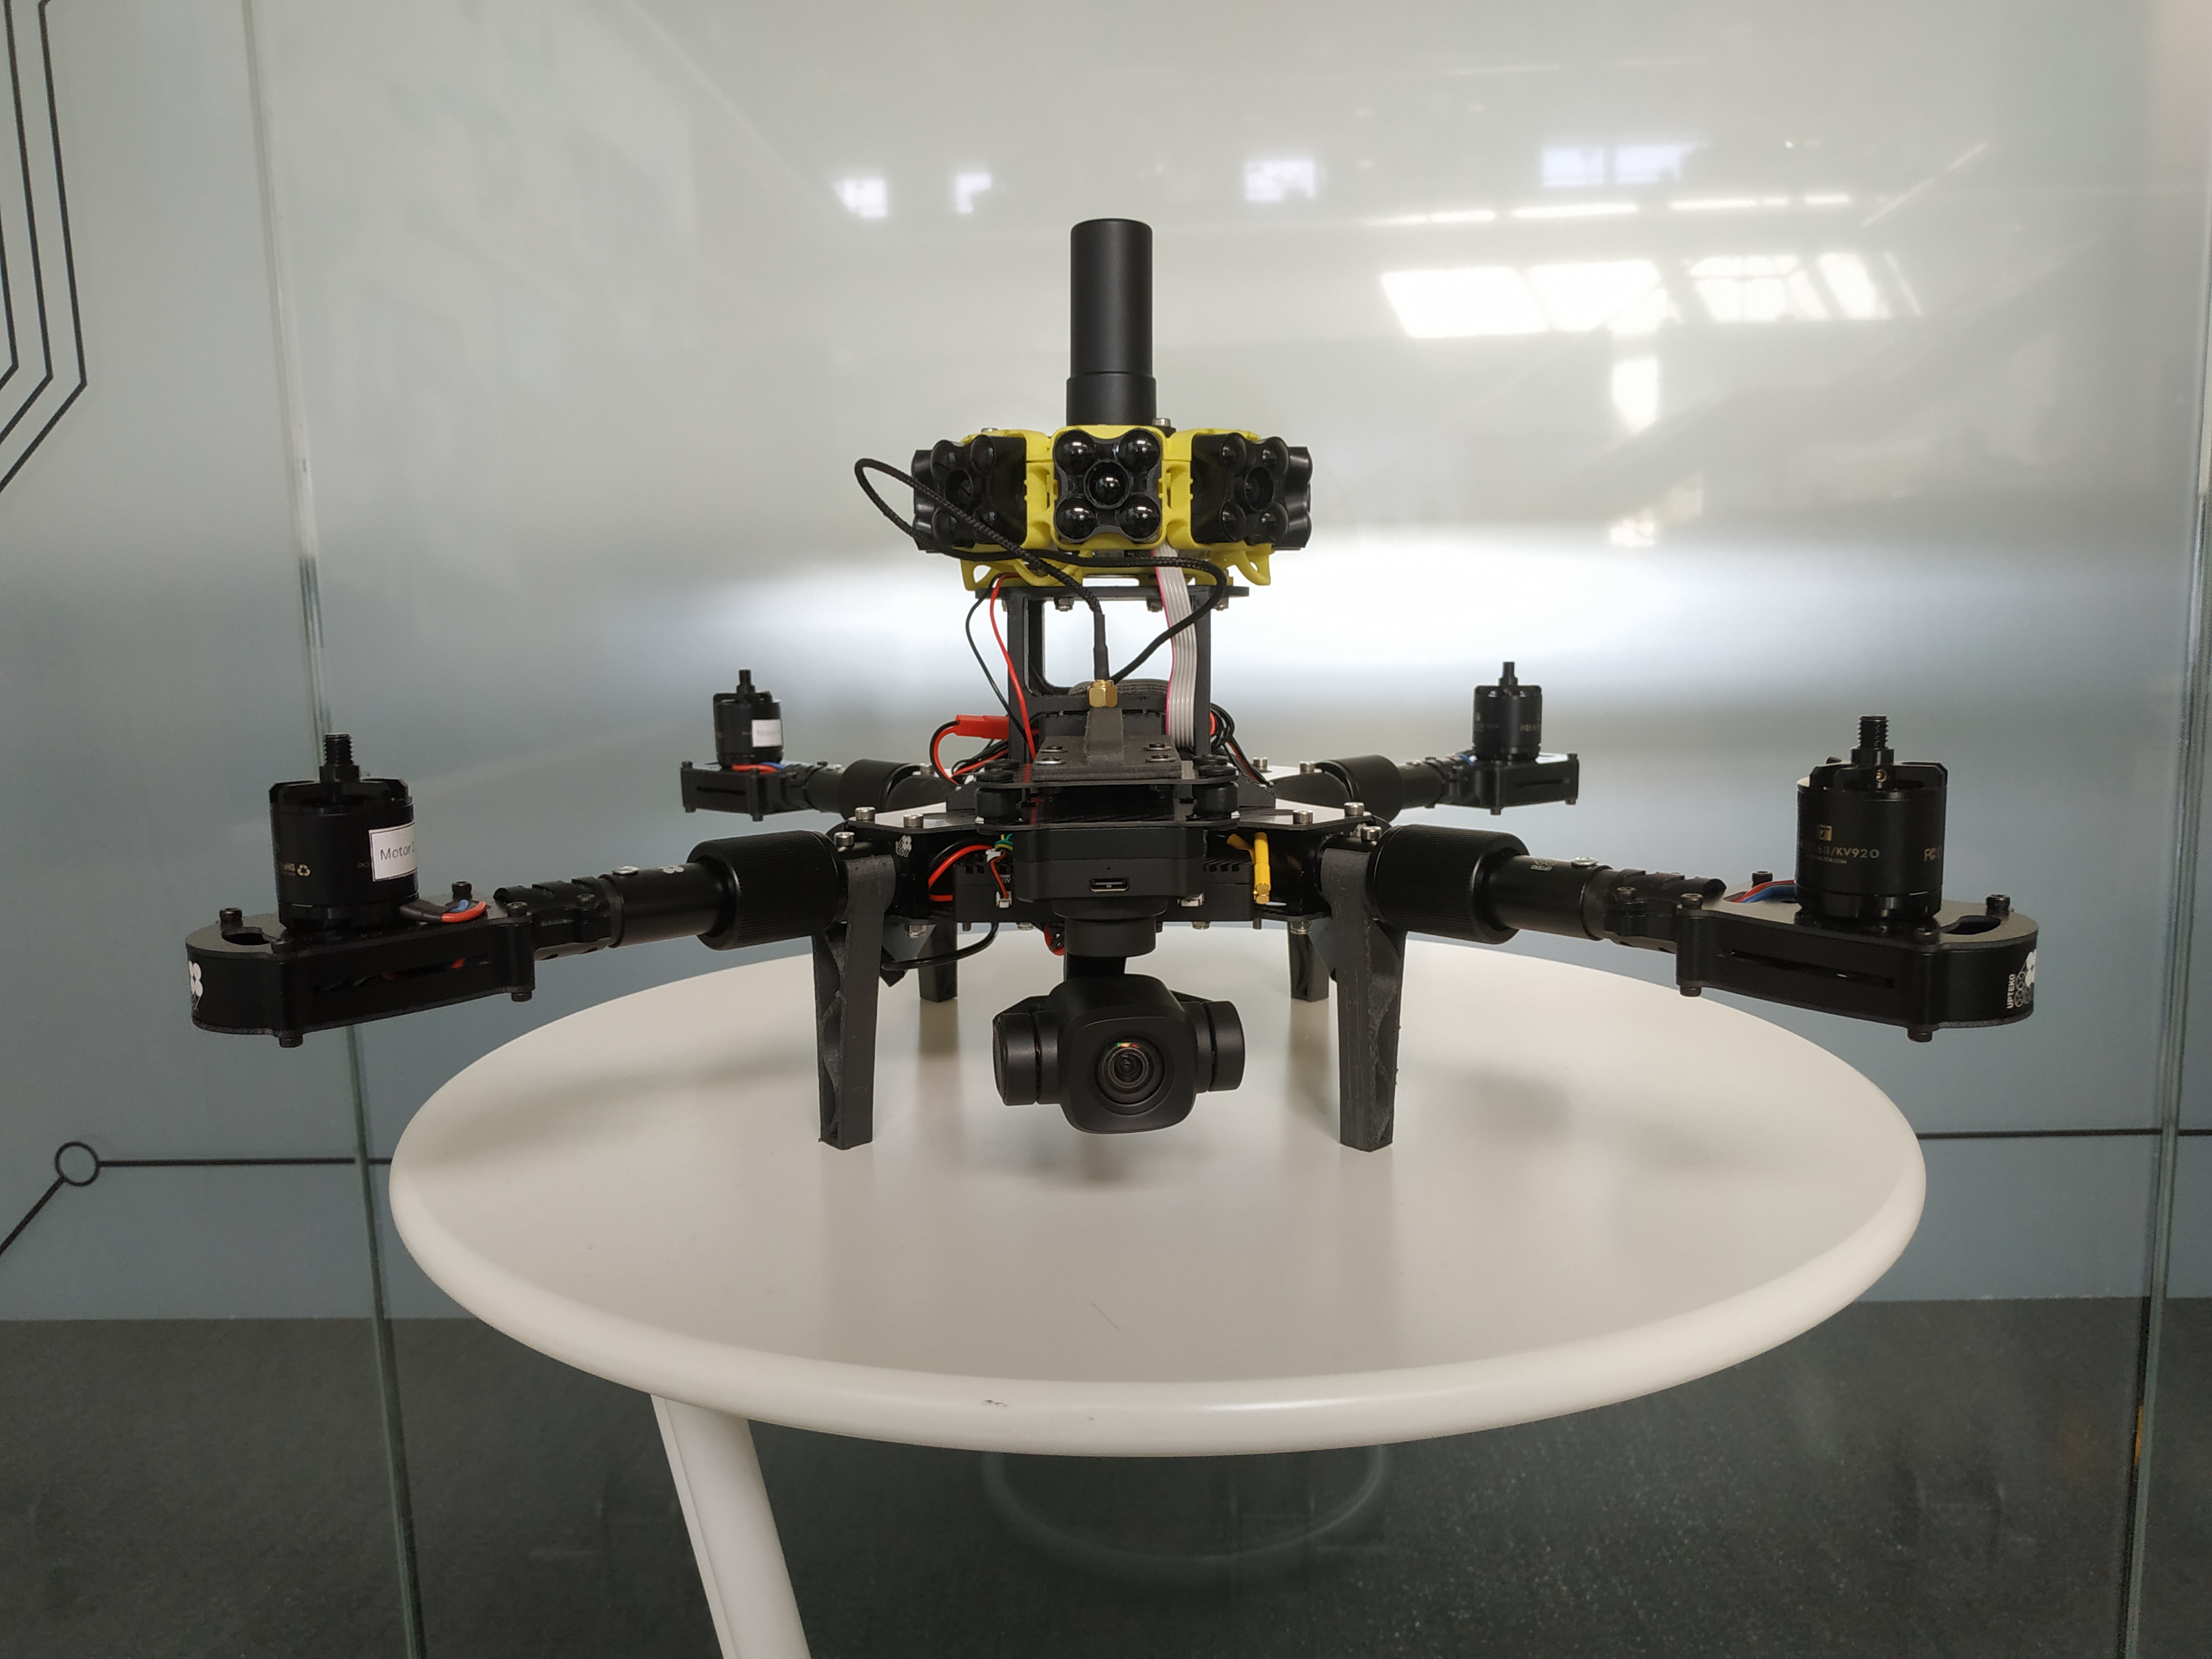
\includegraphics[width=\textwidth]{./projects/logviewer/drone_f_view.jpg}
        \caption{Front view}
    \end{subfigure}
    \hfill
    \begin{subfigure}[b]{0.475\textwidth}   
        \centering 
        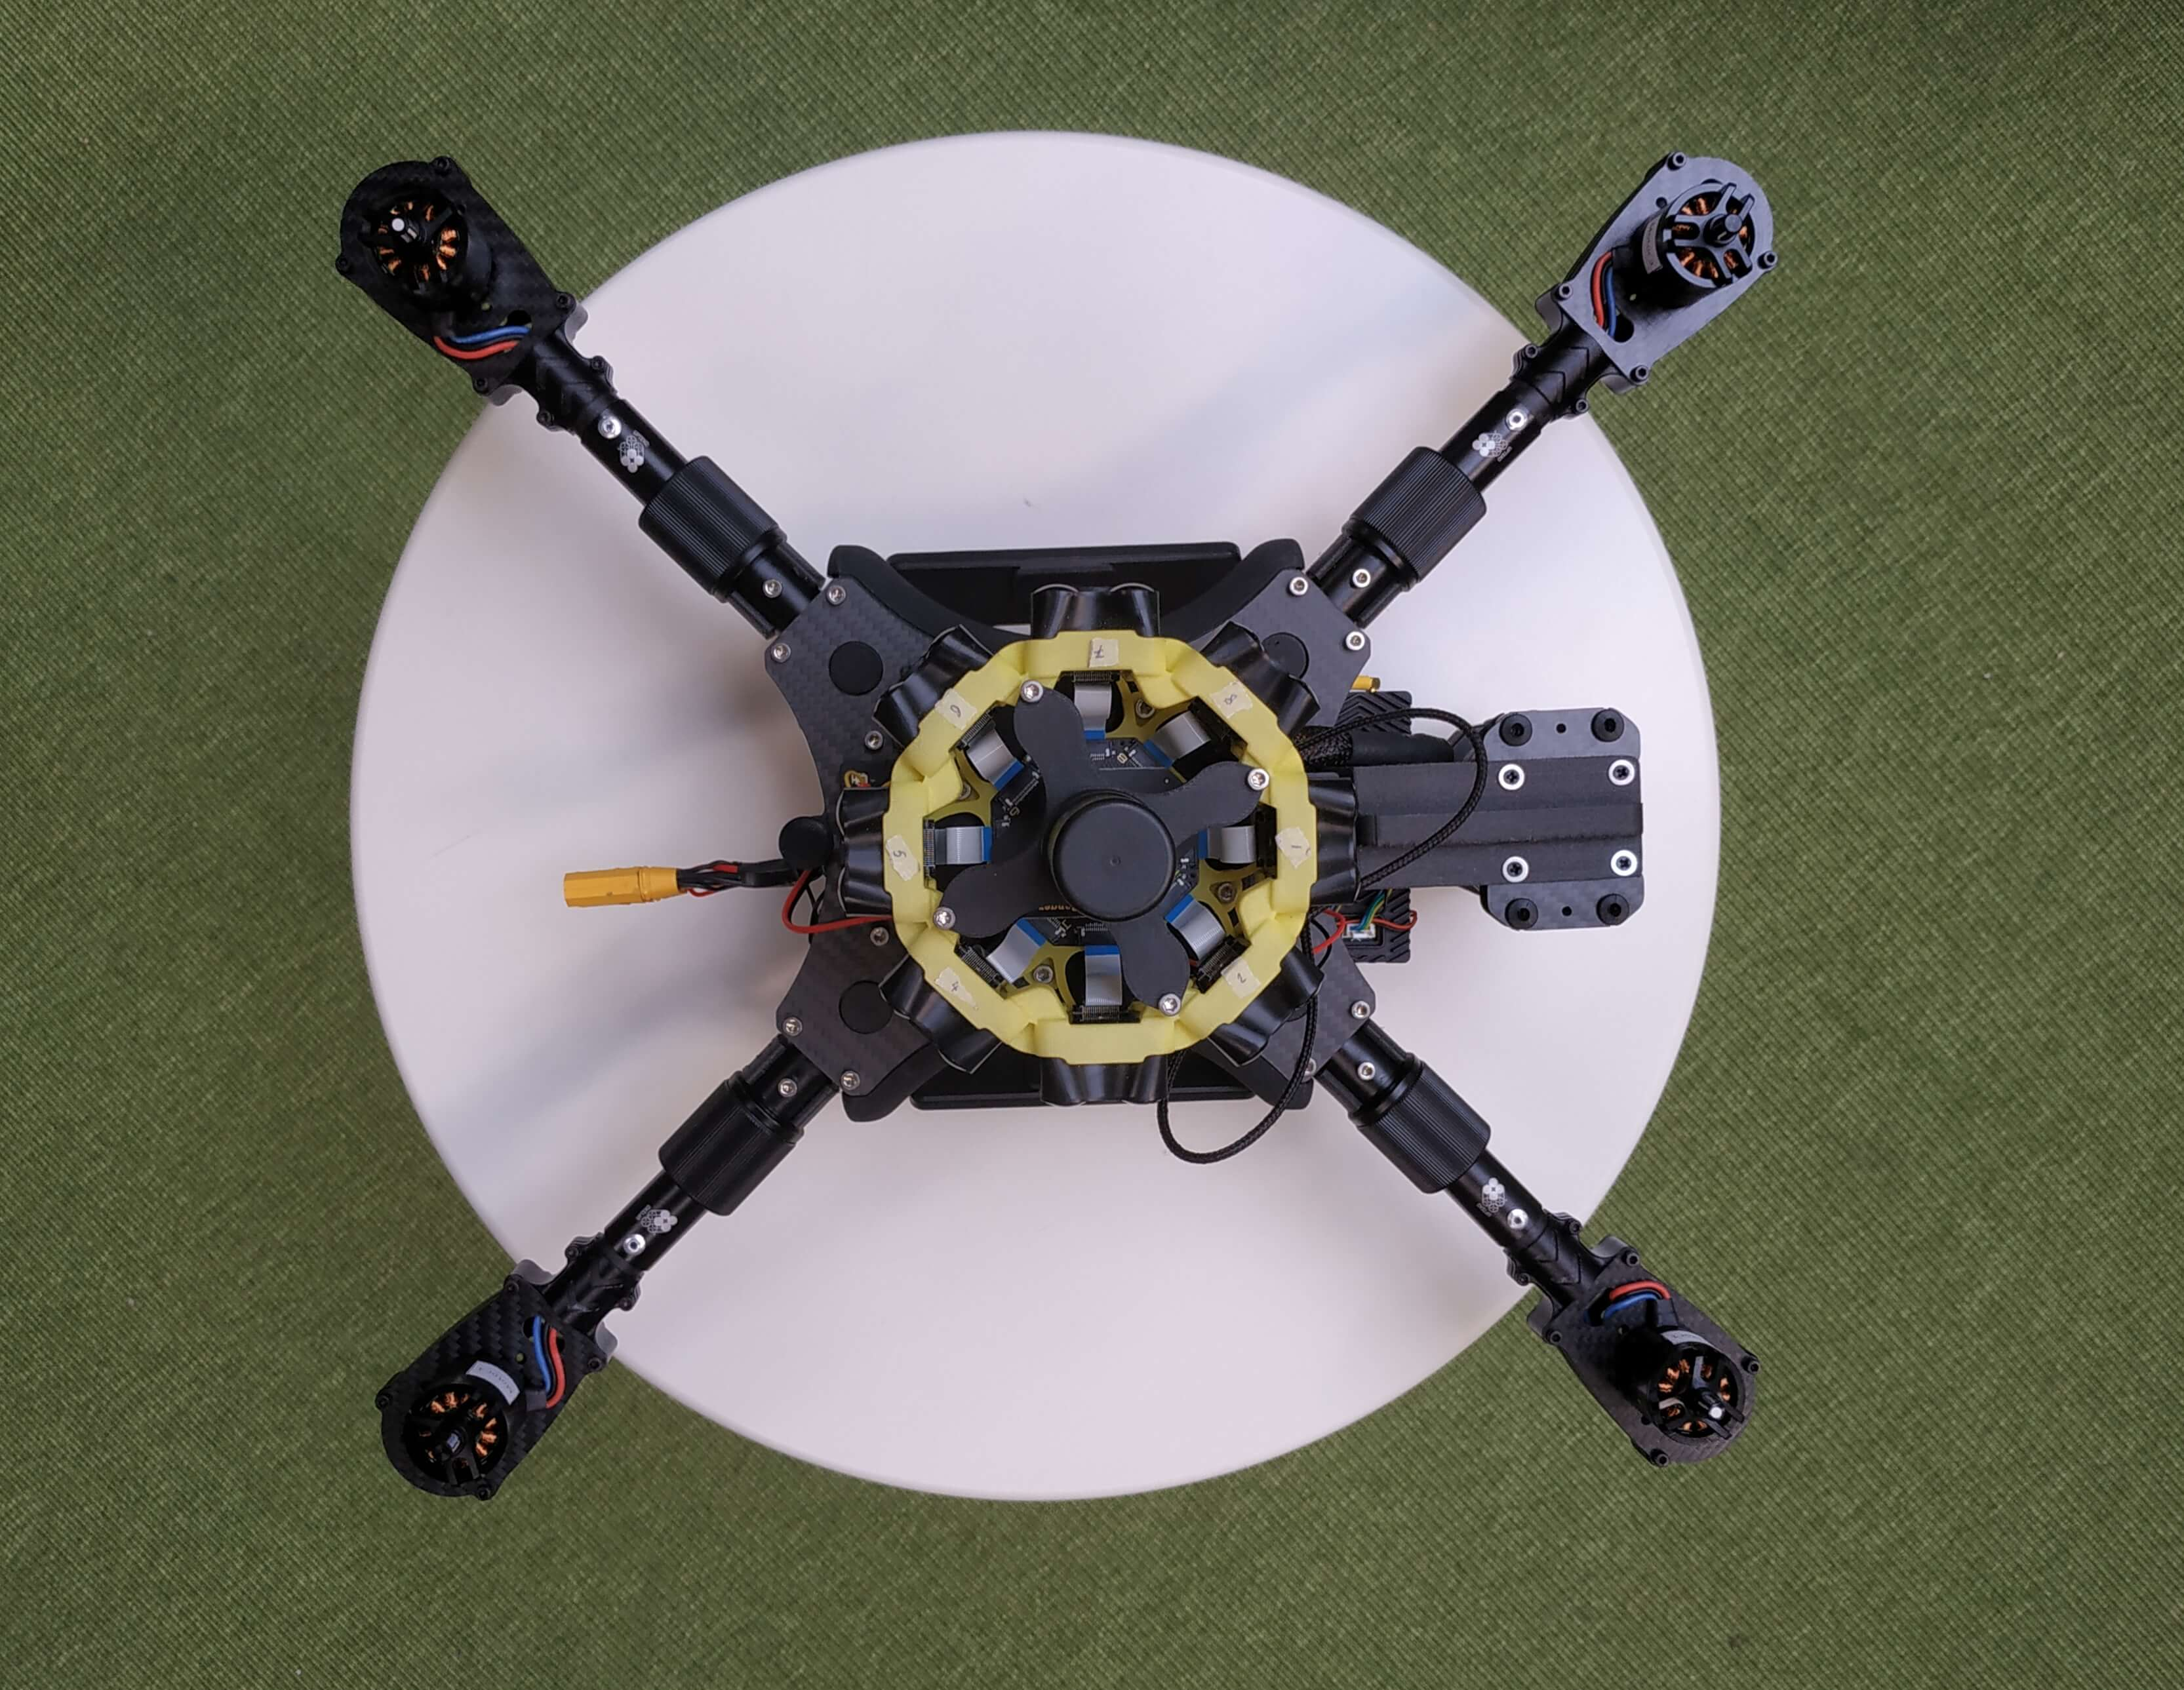
\includegraphics[width=\textwidth]{./projects/logviewer/drone_t_view.jpg}
        \caption{Top view}
    \end{subfigure}
    \caption{Larke Mini drone pictures with 360° degrees \gls{lidar} mounted} 
\end{figure}
The sensors are not integrated into the hull, requiring a large, bulky tower on top of the Larke Mini drone. The integration with the drone is not aesthetic but functional.
\\ \\
Nevertheless the drone successfully achieved its intended mission objectives. Whether it was aerial mapping or surveying, the drone captured distance data effectively.
My colleague Sebastian Duus ensured that the drone was in the optimal position for data acquisition, adjusting altitude and camera settings accordingly.

\subsection{Python Plotly Visualizer}
A graphical user interface is provided, leveraging \texttt{Plotly}\cite{plotly} library. The Logviewer import the \texttt{.csv} file as data.
Here is the \texttt{logfile.csv} header :
\begin{table}[H]
    \centering
    \begin{tabular}{|l|l|l|l|l|l|}
    \hline
    timestamp(ms) & PRX.D0 & PRX.D45 & PRX.D90 & PRX.D135 & PRX.D180 \\
    \hline
    PRX.D225 & PRX.D270 & PRX.D315 & ATT.Roll & ATT.Pitch & ATT.Yaw \\
    \hline
    \end{tabular}
    \caption{Plotly logviewer file header}
    \label{table:logfile_header}
\end{table}

The application is pretty simple : it use the timestamp as main variable to create animated data.
I created 3 main plots in th same window :
\begin{itemize}
    \item the distance sensors plot
    \item the roll and pitch attitude
    \item the yaw plot
\end{itemize}


The most valuable part of this application is the time slider that can be used to go back in time, pause and restart the view.
This way the data analysis is easy-to-use.

\subsubsection{Final result}
\begin{figure}[H]
    \centering
        \href{https://youtu.be/TejnL4hHQNA}{
            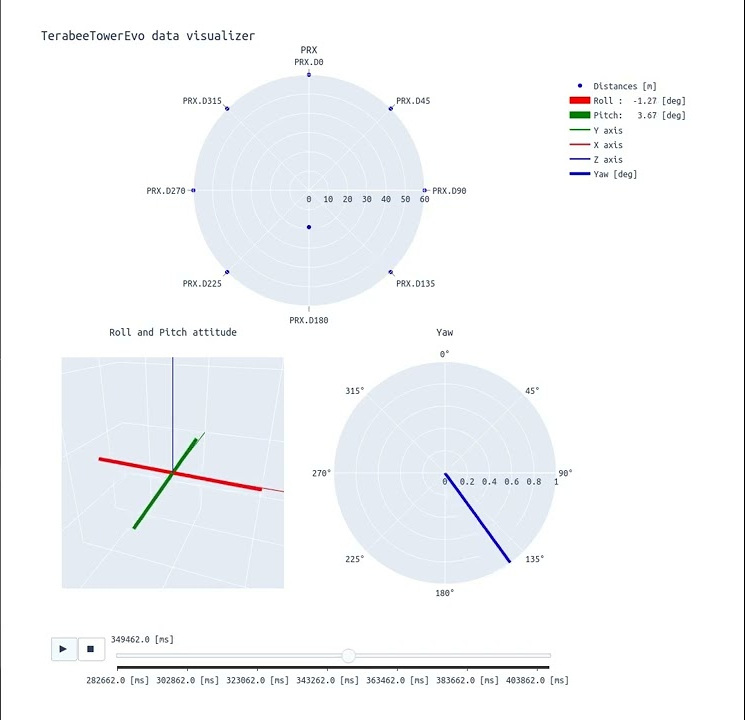
\includegraphics[width=0.5\linewidth]{./projects/logviewer/logviewer_thumbnail.jpg}
        }
        \caption{Python LogViewer demo}
\end{figure}


\section{Collision avoidance SITL}
\subsection{Environement description}
\subsubsection{Robot Operating System}
% ROS2 %
\texttt{\gls{ros2}} is an open-source framework for building robotic systems. It supports distributed systems, allowing communication between different components and nodes running on separate devices.
It provides a communication infrastructure for exchanging messages and supports various protocols. \gls{ros2} introduces a quality of service system for controlling communication behavior.
It includes real-time capabilities for time-critical applications. It supports multiple programming languages and emphasizes modularity and extensibility. ROS 2 comes with development tools and has an active community and ecosystem.
Overall, \gls{ros2} provides a powerful and versatile platform for developing robotic systems. Its distributed architecture, flexible communication infrastructure, real-time capabilities, language support, and extensibility make it a valuable tool for building complex and advanced robots.
\subsubsection{Gazebo}
% gazebo %
\texttt{Gazebo} is an open-source 3D simulation environment for robotics. It allows developers to create virtual worlds where they can simulate and test robots. Gazebo provides realistic physics-based simulations, visualizes the environment in 3D, and simulates sensors like cameras and \gls{lidar}s.
Users can model robots and their surroundings, integrate with the \gls{ros}, and extend its functionality using plugins. Gazebo has a supportive community and offers a wide range of resources for developers.
In summary, Gazebo is a valuable tool for simulating and evaluating robotic systems before deploying them in real-world environments.
\subsubsection{Ardupilot}
% ardupilot %
\texttt{Ardupilot} is open-source software used for controlling autonomous vehicles like drones. It includes firmware that runs on the vehicle's autopilot hardware, as well as ground control station \gls{gcs} software for mission planning and monitoring.
Ardupilot supports different flight modes, navigation based on waypoints, and telemetry for communication with the vehicle. It is compatible with various hardware platforms and can be customized and extended.
Ardupilot is widely used in drones and other vehicles, and it has a supportive community and extensive documentation. In summary, Ardupilot is a versatile and customizable software suite for autonomous vehicle control.

\subsection{Software-In-The-Loop Ardupilot collision avoidance}
The collision avoidance feature in Ardupilot is designed to enhance the safety and reliability of these vehicles by detecting and avoiding potential collisions with obstacles or other aircraft.
\break
The collision avoidance system in Ardupilot relies on various sensors and algorithms to perceive the environment and make informed decisions about navigation. Some of the key components and techniques used in the Built-In Ardupilot collision avoidance include:

\begin{itemize}
    \item \underline{Sensor Inputs:} Ardupilot can interface with different types of sensors, including proximity sensors, \gls{lidar}, sonar, and cameras. These sensors provide information about the surrounding environment and help in detecting obstacles.
    \item \underline{Obstacle Detection:} The collision avoidance system processes the sensor data to identify potential obstacles in the flight path. This can include buildings, trees, other aircraft, or any other objects that may pose a risk of collision.
    \item \underline{Path Planning:} Based on the environment map and the current position of the vehicle, Ardupilot generates a safe and collision-free path for the aircraft to follow. It considers factors such as obstacle proximity, vehicle speed, and maneuverability to calculate an optimal trajectory.
    \item \underline{Collision Avoidance Algorithms:} Ardupilot employs sophisticated algorithms to predict the future movement of obstacles and determine the best course of action to avoid collisions. These algorithms take into account the dynamics of the vehicle and the obstacles.
\end{itemize}
\hfill \break
\gls{sitl} is a testing and simulation technique used in software development and engineering. It involves the integration of software components into a simulated environment or virtual platform to assess their functionality and behavior.
Using it, developers can identify and resolve potential issues and bugs in the software early in the development cycle, reducing costs and risks associated with late-stage failures.
\hfill \break
The Figure~\ref{fig:sitl-overall} represent the non-detailed structure of the work environment and the communication between each of its components :
\begin{figure}[H]
    \centering
    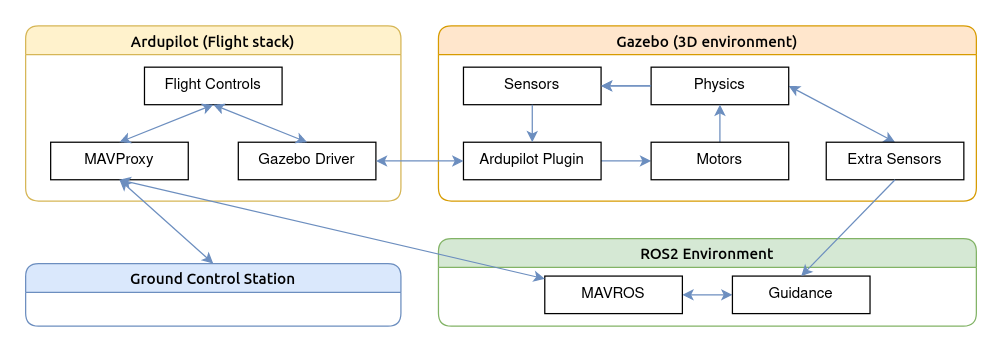
\includegraphics[width=\linewidth]{./projects/ardupilot/sitl_overall.png}
    \caption{Software-In-The-Loop overall chart\cite{sitl_explained}}
    \label{fig:sitl-overall}
\end{figure}

It took a number of steps to obtain a vehicle that could be used in simulation. All the control of the motors and their physical action in Gazebo is already done, but with the integration of the TeraTowerEvo distance sensors.
\\ 
For the sensors to work as realistically as possible, they need to be parameterized in such a way that the minimum and maximum distances correspond to the datasheet, that the angle of vision is also the same, and to add a little noise to the measurements captured.
\\ \\
Once everything is set up, the data can be easily analyzed in the integrated ROS interface (cf. Figure~\ref{fig:drone-gazebo}):
\begin{figure}[H]
    \centering
    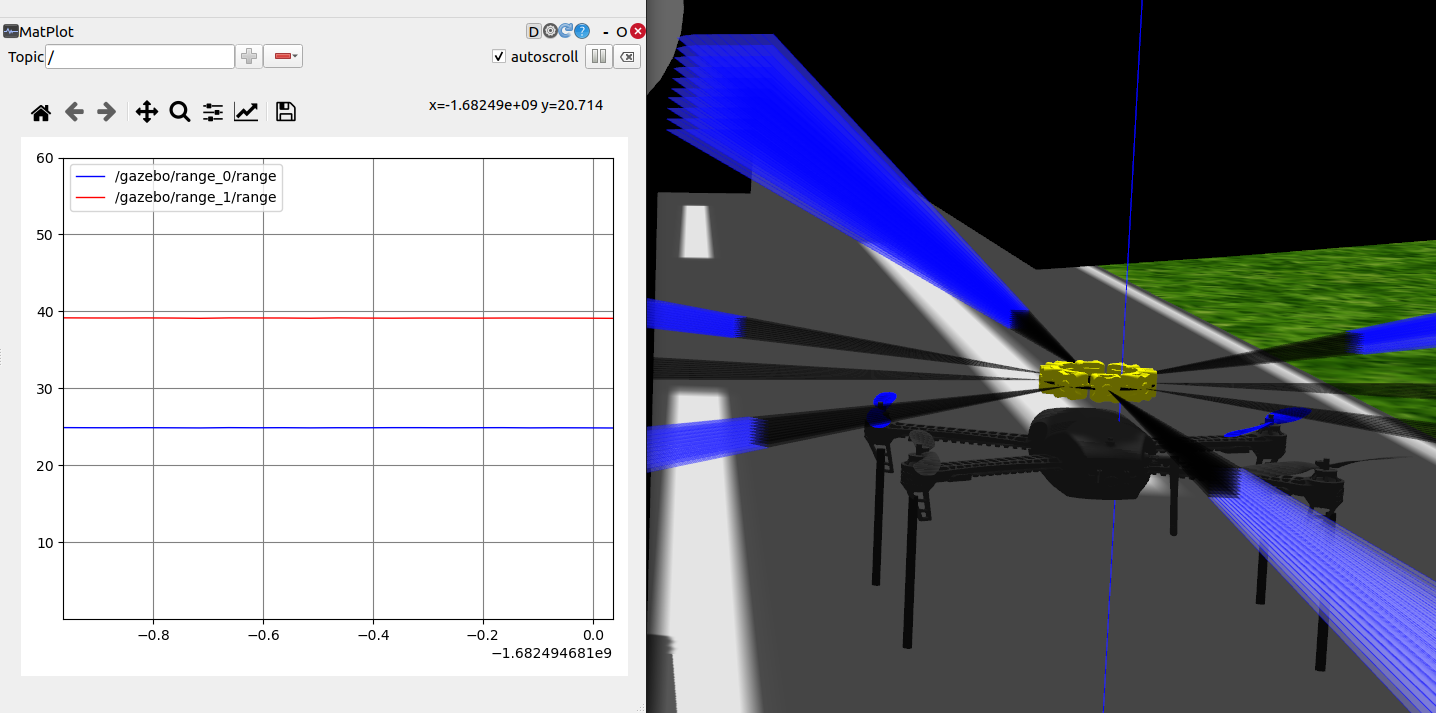
\includegraphics[width=0.75\linewidth]{./projects/ardupilot/gazebo_drone.png}
    \caption{Drone with TowerEvo in Gazebo environment}
    \label{fig:drone-gazebo}
\end{figure}

\subsection{Collision Avoidance ROS2 Migration}
\subsubsection{ ROS1 collision-avoidance description}

The aim of this task is to migrate a project from the old version of Robot Operating System (\gls{ros}) to the new one \gls{ros2}.

\begin{wrapfigure}{l}{0.55\textwidth}
    \centering
    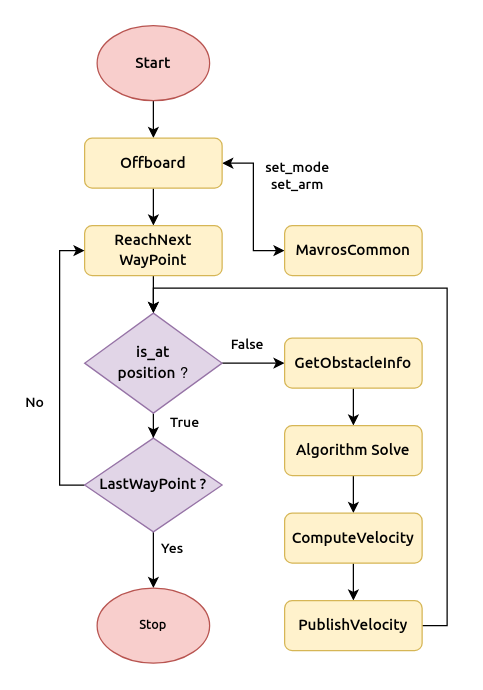
\includegraphics[width=0.45\textwidth]{./projects/ardupilot/ca_flowchart.png}
    \caption{Collision Avoidance flowchart}
    \label{fig:ca-flowchart}
\end{wrapfigure}

\hfill \break
The Figure~\ref{fig:ca-flowchart} represent how the collision avoidance logic is working.
It's basically a loop that covers all the waypoints to reach the final destination.The data acquired by the distance sensors are continuously recorded to enable the algorithm to detect obstacles and change the speed and direction of the drone in real time.
As soon as data are acquired, this action chain start : \texttt{GetObstacleInfo}, \texttt{Algorithm Solve}, \texttt{ComputeVelocity} and \texttt{PublishVelocity}.
\hfill \break
\hfill \break
It use the \texttt{potential field method}\cite{potential_field}, it's an algorithm used in robotics for motion planning. It represents the environment as a field of attractive and repulsive potentials. The agent is guided towards the goal by attractive potentials and repelled by repulsive potentials generated by obstacles. The agent follows the gradient of the potential field to navigate towards the goal while avoiding obstacles.
It is a simple and intuitive approach but can have limitations in complex environments and local minima trapping. Extensions and modifications exist to address these challenges.

\subsubsection{ROS migration}
Migration is a complex process that requires a thorough understanding of the environment in which you're moving and the environment in which you're moving. What's more, programming languages (python here) often evolve between 2 ROS releases, so language errors add to the difficulty.
I successfully migrate all the files as espected but unfortunatly after 3 weeks working on this tasks, I wasnt able to debug and test the project due to the environment complexity.
\\ \\
My colleagues are way more experienced in ROS2 and migration, so we decided together to stop my part here and let them continue to debug and test the project.\\
I did, however, learn a lot of principles, such as \gls{qos} and \gls{mavlink} message communication, which are essential for flying robotics projects.
